\documentclass{awac02}

% Packages
\usepackage[utf8]{inputenc}
\usepackage{tabularx}
\usepackage{graphicx}
\usepackage{svg}
\usepackage{tikz}
\usepackage{xparse}
\usetikzlibrary{positioning, fit, backgrounds, shapes, arrows.meta}

% State machine

\tikzstyle{base} = [minimum width=3cm, minimum height=1cm, node distance=2em, text centered, draw=black, inner sep=5pt]

\tikzstyle{start} = [base, rectangle, rounded corners, draw=black, fill=red!30]

\tikzstyle{io} = [trapezium, trapezium left angle=70, trapezium right angle=110, 
 minimum height=1cm, text centered, draw=black, fill=blue!30, trapezium stretches=true,
 align=center, inner sep=1em] 

\tikzstyle{state} = [base, rectangle, fill=orange!30]

\tikzstyle{decision} = [base, rectangle, rounded corners=0.8em, fill=green!30]

\tikzstyle{subprocess} = [rectangle, draw = black!50, minimum height = 2em, fill=pink!50]

\tikzstyle{process2} = [rectangle, minimum height=1cm, align=center, draw=black, fill=yellow!30, inner sep=1.8em]

\tikzstyle{process_label} = [external/.style={draw=black!50}, font={\fontsize{13pt}{12}\selectfont}]

\tikzstyle{arrow} = [thick,->,>=stealth]
\tikzstyle{slow_arrow} = [dotted, thick,->,>=stealth]
\tikzstyle{line} = [thick]

\NewDocumentCommand\StateWithBullets{m m m >{\SplitList{;}}m}{%
    \node (#1) [state, text width=6cm, #2, inner sep=5pt] {\large #3\small \begin{itemize}
    \ProcessList{#4}{\insertitem} \end{itemize}};
}
\newcommand\insertitem[1]{\item #1}

\NewDocumentCommand\JustBullets{m m >{\SplitList{;}}m}{%
    \node (#1) [state, text width=3.5cm, #2, inner sep=5pt, rounded corners,
    fill=blue!30] {\vspace{-0.8em}\small\begin{itemize}
    \ProcessList{#3}{\insertitem} \end{itemize}};
}

% Distances
\newcommand{\shortarrowlength}{3.1em}

% Menu
\tikzstyle{menu-base} = [text centered, draw=black, inner sep=0.5em, node
distance=4em, minimum height=3em, minimum width=9em]

\tikzstyle{menu-enterexit} = [menu-base, rectangle, rounded corners, fill=black!10]

\tikzstyle{menu-item} = [menu-base, rectangle, rounded corners, minimum height=3.5em]

\tikzstyle{menu-small-item} = [menu-base, rectangle, rounded corners, minimum
width=4em, minimum height=2em]

\tikzstyle{menu-setting} = [menu-base, rectangle, rounded corners, minimum
width=7em]

\tikzstyle{button-label} = [circle, draw=black, minimum size=1.3em, fill=white, inner
sep=0, line width=0.5pt, font=\footnotesize]

\tikzstyle{menu-single} = [->, >={Latex[length=2mm, width=3mm]}, line width=4pt]
\tikzstyle{menu-double} = [menu-single, <->]

\newcommand{\LRvert}[2]{%
    \draw[menu-single] ([xshift=1em]#1.south) -- node[button-label] {R}
        ([xshift=1em]#2.north);
    \draw[menu-single] ([xshift=-1em]#2.north) -- node[button-label] {L}
        ([xshift=-1em]#1.south);
}

\newcommand{\LRhor}[2]{%
    \draw[menu-single] ([yshift=0.5em]#1.east) -- node[button-label] {R}
        ([yshift=0.5em]#2.west);
    \draw[menu-single] ([yshift=-0.5em]#2.west) -- node[button-label] {L}
        ([yshift=-0.5em]#1.east);
}

\newcommand{\IncrementDecrementNode}[2]{%
    \node (_#2anchor) [#1=\shortarrowlength+1.3em of #2, outer sep=1pt, inner sep=0] {};
    \node (_#2L) [button-label, above left=0.2em of _#2anchor] {L};
    \node (_#2dec) [below left=0.2em of _#2anchor, inner sep=0, circle, minimum size=1.3em] {--};
    \node (_#2R) [button-label, above right=0.2em of _#2anchor] {R};
    \node (_#2inc) [below right=0.2em of _#2anchor, inner sep=0, circle, minimum size=1.3em] {+};
    \node (_#2set) [fit={(_#2L) (_#2R) (_#2dec) (_#2inc)}, draw] {};
}

\newcommand{\SetTimeNode}[3]{%
    \node (#1) [#2, menu-small-item] {#3};
    \IncrementDecrementNode{below}{#1}
    \draw[menu-double] (#1) -- node[button-label] {SP} (_#1set.north);
}



\title{Documentation}
\begin{document}

\maketitle

\section{Overview}

The documentation is meant as a guide for the developer. Additional aid is
found in the source header files where most functions are documented.

\section{Source Files}

In this section an overview of the project files are given.
The files are listed in order of relevance.

\begin{centering}
\vspace{3mm}
\begin{tabularx}{.9\textwidth}{ >\raggedright p{5cm} | X }
    File(s)                  & Description \\ [0.5ex]
    \hline
    \texttt{main.c}                     & The main file. Contains the
                                          clock-mode state-machine.\\
    \texttt{constants.h}                & Global constants for defining number
                                          of displays, enabling logging etc. \\
    \texttt{menu.h}, \texttt{menu.c}    & The state machine for the menu. \\
    \texttt{utilities.h}, \texttt{utilities.c} & High level utilities. Mostly
                    for applying and showing settings. \\
    \texttt{log.h}, \texttt{log.c}      & Logging functions. Everything here
                                          will be unavailable if the LOG
                                          constant is undefined. \\
    \texttt{rtc.h}, \texttt{rtc.c}      & High level functions to set and show
                                          the external RTC clock. \\
    \texttt{display.h}, \texttt{display.c} & Low level functions to interface
                                             with the Qwiic Alphanumeric Display \\
    \texttt{helpers.h}, \texttt{helpers.c} & Simple helper-functions. \\
    \texttt{external\_interrupts.h}, \texttt{external\_interrupts.S} &
                    Register and extract the external interrupts (button
                    presses and RTC alarms). \\
    \texttt{time.h}, \texttt{time.S}    & Start and use the hardware times. \\
    \texttt{twi.h}, \texttt{twi.S}      & Interface to the TWI (I2C) hardware.
                                          Read and write to external devices. \\
    \texttt{eeprom.h}, \texttt{eeprom.S} & Read and write to the EEPROM
                                           (non-volatile storage). \\
    \texttt{flash.h}, \texttt{flash.S}  & Read constant data from flash. For
                                          example an ASCII conversion table. \\
    \texttt{io.h}, \texttt{io.S}        & Direct control of pins. \\
    \texttt{usart.h}, \texttt{usart.S}  & Send data through USART. This is used
                                          to implement printf in `log.c` \\
    \texttt{math.S}                     & Low level math for assembly routines.
\end{tabularx}
\end{centering}

\section{Schematic}

In figure \ref{fig:circuit} the circuit is shown. The value of R1-R7, C1 and C5-C7
is only approximate. You can try different values. In addition to these
components two Sparkfun Qwiic Alphanumeric Displays are used. One of the
displays must be modified to disable the pull-up resistors and change the slave
address to \texttt{0x71}.

\begin{figure}[h]
    \centering
    \includegraphics[width=\textwidth, trim=5cm 5cm 6cm 2cm, clip]{../Circuit}
    \caption{The circuit (excluding displays).}
    \label{fig:circuit}
\end{figure}

\section{State Machine}

The state machine for clock mode is in \texttt{main.c} and the state machine
for the menu mode is in \texttt{menu.c}. They are implemented using the
\texttt{goto} statement which can lead to hard to understand code.  To give the
programmer a better overview of the states and make development easier some
states are documented here and shown in flow-charts. The program starts in the
\texttt{enter\_clock\_mode} state. The clock mode state machine is illustrated
in Figure \ref{fig:clock-state}.

\begin{figure}[h]
    \centering
    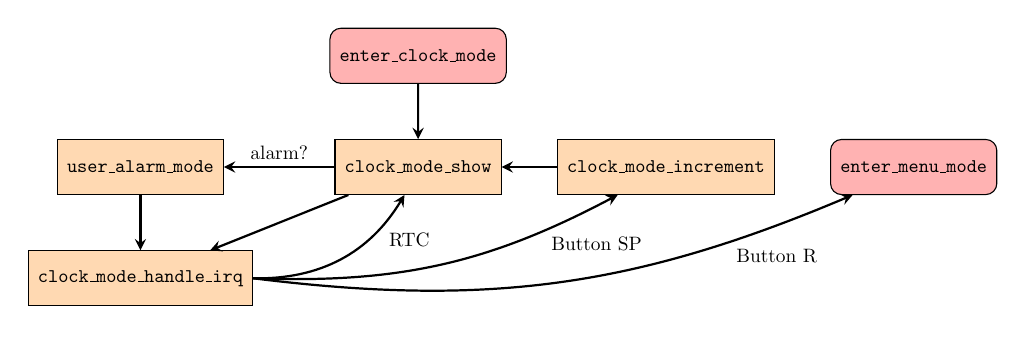
\begin{tikzpicture}[every node/.style={scale=0.7}]

\node (CLOCK_MODE_SHOW) [state] { \texttt{clock\_mode\_show}};
\node (USER_ALARM_MODE) [state, left=4em of CLOCK_MODE_SHOW] {\texttt{user\_alarm\_mode}};
\node (ENTER_CLOCK_MODE) [start, above=of CLOCK_MODE_SHOW] {\texttt{enter\_clock\_mode}};
\node (CLOCK_MODE_INCREMENT) [state, right=of CLOCK_MODE_SHOW] {\texttt{clock\_mode\_increment}};
\node (HANDLE_IRQ) [state, below=of USER_ALARM_MODE] {\texttt{clock\_mode\_handle\_irq}};
\node (ENTER_MENU_MODE) [start, right=of CLOCK_MODE_INCREMENT] {\texttt{enter\_menu\_mode}};


\draw [arrow] (ENTER_CLOCK_MODE) -- (CLOCK_MODE_SHOW);

%\draw [arrow] (CLOCK_MODE_CHECK_INTERRUPTS) -| node[anchor=north]{RTC}
%    (CLOCK_MODE_SHOW);
%\draw [arrow] (CLOCK_MODE_CHECK_INTERRUPTS) -| node[anchor=north]{Button SP} (CLOCK_MODE_INCREMENT);
%\draw [arrow] (CLOCK_MODE_CHECK_INTERRUPTS) -| node[anchor=north]{Button R} (ENTER_MENU_MODE);

\draw [arrow] (CLOCK_MODE_SHOW) -- node [midway, above] {alarm?} (USER_ALARM_MODE);
\draw [arrow] (CLOCK_MODE_SHOW) -- (HANDLE_IRQ);
\draw [arrow] (CLOCK_MODE_INCREMENT) -- (CLOCK_MODE_SHOW);

\draw [arrow] (USER_ALARM_MODE) -- (HANDLE_IRQ);

\draw [arrow] (HANDLE_IRQ.east) to [bend right=30]
node[anchor=north west, pos=0.8] {RTC} (CLOCK_MODE_SHOW);

\draw [arrow] (HANDLE_IRQ.east) to [bend right=15]
node[anchor=north west, pos=0.8] {Button SP} (CLOCK_MODE_INCREMENT);

\draw [arrow] (HANDLE_IRQ.east) to [bend right=15]
node[anchor=north west, pos=0.8] {Button R} (ENTER_MENU_MODE);

\end{tikzpicture}

    \caption{The clock mode state machine}
    \label{fig:clock-state}
\end{figure}

The menu mode state machine is a bit more complicated. A simple overview is
shown in Figure \ref{fig:menu-flowchart}. There are three basic state types in the
menu. \emph{Menu} states, \emph{choose} states and \emph{set} states. The menu
states are very simple. Each show some text on the display, then wait for a
button interrupt. If the \texttt{L} or \texttt{R} button is pressed the
state is changed to the previous or next menu state. If the \texttt{SP} button
is pressed it is changed to a choose or set state.

A choose state is used when there is multiple options for the setting that is
edited. For example when changing time. A choose state first shows the current
value of that setting, sets an RTC alarm for when it is changed and waits for
an interrupt. If the interrupt is from the RTC the new value is shown. If it is
from the \texttt{L} or \texttt{R} buttons the state changes to the previous or
next choose state. If it is from the \texttt{SP} button the state changes to
the corresponding set state.

A set state works a lot like a choose state. A RTC interrupt changes the value
shown and \texttt{SP} interrupt changes state (go back to the choose state).
But a \texttt{L} or \texttt{R} button interrupt de- or increments the value
instead.

Figure \ref{fig:choose-and-set-state} shows the program flow between a choose
and a set state in detail. The actual implementation varies slightly
between types.

\begin{figure}[h]
    \centering
    \begin{tikzpicture}[every node/.style={scale=1}]


\StateWithBullets{CHOOSE}{draw}{Choose state}{Set left display (show type);Set
    right display (show value);Arm
RTC alarm for value change}

\JustBullets{RTC1}{above=of CHOOSE}{Arm RTC alarm; Update right display}

\JustBullets{SET_DONE}{below=of CHOOSE, xshift=4em}{Disable display blink mode}

\StateWithBullets{SET}{below=3 of CHOOSE}{Set state}{Set right display blink mode}

\node (PREVIOUS) [left=of CHOOSE] {Previous choose state};
\node (NEXT) [right=of CHOOSE] {Next choose state};

\JustBullets{DEC}{left=of SET}{Decrement value;Set right display}
\JustBullets{INC}{right=of SET}{Increment value;Set right display}
%\node (INC) [right=of SET, text width=8em] {Increment value, \\ Set right display};

\JustBullets{RTC2}{below=of SET}{Arm RTC alarm; Update right display}

% Arrows
\draw[arrow] (CHOOSE) -- node[anchor=south] {\texttt{L}} (PREVIOUS);
\draw[arrow] (CHOOSE) -- node[anchor=south] {\texttt{R}} (NEXT);
\draw[arrow] (CHOOSE) -- node[anchor=east] {\texttt{RTC}} (RTC1);

\draw[arrow] ([xshift=-4em]CHOOSE.south) -- node[anchor=east] {\texttt{SP}}
    ([xshift=-4em]SET.north);

\draw[arrow] ([xshift=4em]SET.north) -- node[anchor=east] {\texttt{SP}}
    (SET_DONE.south);
\draw[arrow] (SET_DONE.north) -- ([xshift=4em]CHOOSE.south);

\draw[arrow] (SET) -- node[anchor=south] {\texttt{L}} (DEC);
\draw[arrow] (SET) -- node[anchor=south] {\texttt{R}} (INC);
\draw[arrow] (SET) -- node[anchor=east] {\texttt{RTC}} (RTC2);

%\node (TESTNODE) [draw, text width=3cm] {Hejsvejs \newline $\bullet$ title};

%\node [font=\Large] (top)    at (5,10) {Choose state};
%\node [font=\Large] (middle) at (5,9)  {$\bullet$ [1]};
%\node [font=\Large] (bottom) at (5,8)  {$\bullet$ [2]};
%\node[draw=brown, thick,fit={(top) (middle) (bottom)}, inner sep=10pt]   (box) {};

\end{tikzpicture}

    \caption{A choose and set state combo}
    \label{fig:choose-and-set-state}
\end{figure}

\begin{figure}[h]
    \centering
    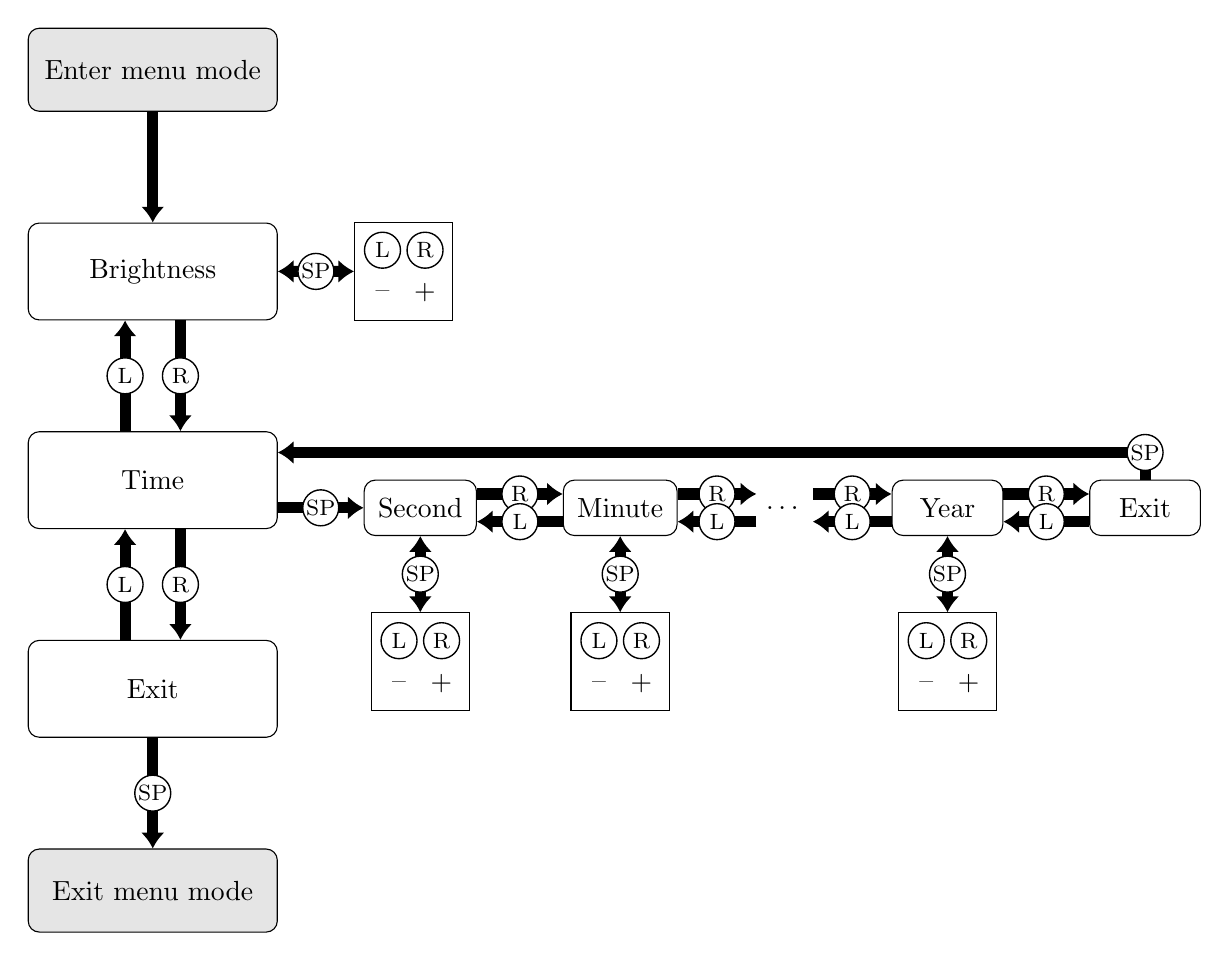
\begin{tikzpicture}[every node/.style={scale=1}]

\node (ENTER_MENU_MODE) [menu-enterexit] { Enter menu mode };

\node (MENU_BRIGHTNESS) [menu-item, below=of ENTER_MENU_MODE] { Brightness };

\IncrementDecrementNode{right}{MENU_BRIGHTNESS}
%\node(SET_BRIGHTNESS) [menu-setting, right=of MENU_BRIGHTNESS] { Set Brightness };

\node(MENU_TIME) [menu-item, below=of MENU_BRIGHTNESS] { Time };

\node(MENU_EXIT) [menu-item, below=of MENU_TIME] { Exit };

\node(EXIT_MENU_MODE) [menu-enterexit, below=of MENU_EXIT] { Exit menu mode };

% Time

\SetTimeNode{SET_SECOND}{right=\shortarrowlength of MENU_TIME,yshift=-1em}{Second};
\SetTimeNode{SET_MINUTE}{right=\shortarrowlength of SET_SECOND}{Minute};

\node (SET_DOTDOTDOT) [right=of SET_MINUTE]{\dots};

\SetTimeNode{SET_YEAR}{right=of SET_DOTDOTDOT}{Year};

\node (SET_EXIT) [menu-small-item, right=\shortarrowlength of SET_YEAR] {Exit};

% Time arrows
\LRhor{SET_SECOND}{SET_MINUTE}
\LRhor{SET_MINUTE}{SET_DOTDOTDOT}
\LRhor{SET_DOTDOTDOT}{SET_YEAR}
\LRhor{SET_YEAR}{SET_EXIT}

% Arrows between menu items
\draw[menu-single] (ENTER_MENU_MODE) -- (MENU_BRIGHTNESS);

\LRvert{MENU_BRIGHTNESS}{MENU_TIME}
\LRvert{MENU_TIME}{MENU_EXIT}

\draw[menu-single] (MENU_EXIT) -- node[button-label] {SP} (EXIT_MENU_MODE);

% Arrows to set brightness items
\draw[menu-double] (MENU_BRIGHTNESS) -- node[button-label] {SP} (_MENU_BRIGHTNESSset);

% Arrows to set time items
\draw[menu-single] ([yshift=-1em]MENU_TIME.east) -- node[button-label] {SP} (SET_SECOND);

\draw[menu-single] (SET_EXIT.north) |- node[button-label] {SP} ([yshift=1em]MENU_TIME.east);

\end{tikzpicture}

    \label{fig:menu-flowchart}
    \caption{An overview of the menu}
\end{figure}

\end{document}
